\chapter{Iteración 3: Primer prototipo de Hardware} % (fold)
\label{cha:iteracion_3}


\section{Introducción} % (fold)
\label{sec:introduccion}

Una vez terminada la iteración 1 (donde definimos los componentes físicos a utilizar), y teniendo en cuenta que en el Laboratorio de Arquitectura de Computadoras (LAC) había una placa de desarrollo de SiliconLabs (modelo C8051f352DK) con gran cantidad de los componentes que nosotros necesitábamos para nuestro desarrollo. Lo que decidimos fue basar y adaptar nuestro diseño a la C8051f352DK, para minimizar los errores.

En esta iteración realizamos el diseño y construcción de una placa de desarrollo que cumpla con los requerimientos planteados.


%la primera placa que fue una verga. tenia el rs232, tenia 8 entradas, tenia la alimentacion separada de la entrada para la programacion del micro. osea podia alimentarse mediante el debugger o alimentacion externa. se adapto el diseño de la placa para poder programar el micro con el debugger de silicon labs. hay que tener en cuenta que nos basamos en el diseño hecho por silicon labs de la placa de desarrollo c8051f352 que teniamos en el lac. la vamos a haber construido en esta iteracion, y lo unico que llego a hacer fue conectarse con la ide. nada mas, el resto no anduvo nada. %

% section introduccion (end)

\section{Requerimientos de la iteracion} % (fold)
\label{sec:requerimientos_de_la_iteracion}

Diseñar y construir un prototipo de placa con las siguientes características:

\begin{itemize}
\item El circuito debe incluir en su diseño aquellos requisitos de hardware impuestos por el mismo microcontrolador(?)
\item Al circuito se le deben poder conectar 8 entradas analógicas.
\item Al circuito se le deben poder conectar 4 entradas de eventos digitales externos.
\item Las entradas analógicas deben tener filtros para mejorar la inmunidad al ruido.
\item Se debe incluir en el diseño el circuito necesario para soportar comunicación vía RS232
\item La placa debería poder alimentarse a través de una fuente de tensión externa.
\item Se debería poder conectar el debugger del microcontrolador a la placa para poder programarlo.
\item El circuito de programación del microcontrolador debería estar separado la placa principal.
\end{itemize}


% section requerimientos_de_la_iteracion (end)

\section{Desarrollo} % (fold)
\label{sec:desarrollo}

\subsection{Elección de Herramientas para Diseño} %(fold)
\label{sec:herramientas_para_diseno}

Gracias a que en el LAC en dicho momento estaba realizando trabajos Santiago Rodriguez (Ingeniero en Computación, egresado de la UNC), pudimos consultar con él sobre el diseño y desarrollo de placas PCB. 

Santiago nos recomendó utilizar varias herramientas para el diseño:
\begin{itemize}
\item Kicad.
\item Altium Designer.
\item Eagle.
\item PCBwizard.
\end{itemize}

Ademas para poder realizar la impresión de la placa PCB en la fresadora que tiene el LAC, ProtoMat E33 de LPKF, necesitamos tener instalado el software de la empresa, llamado LPKF Circuit Pro PM.

Luego de probar las herramientas para diseñar la placa, nos terminamos decidiendo por Kicad, ya que fue el mas sencillo de utilizar, mas amigable su interfaz y era el que nos exportaba los archivos que necesitábamos para poder utilizar el Circuit Pro e imprimir la placa en la Fresadora.

%subsection herramientas_para_diseno (end)

\subsection{Diagramas de Bloques de Hardware}
\label{diagra_bloques_hardware}

La primera etapa de diseño consiste en realizar un diagrama de bloques que, en base a los requerimientos planteados para esta iteración, ilustre a grandes rasgos la organización del circuito que pretendemos realizar.
Podemos ver en la figura \ref{fig:BloquesHardw1} el diagrama de bloque que hicimos.

\begin{figure}[h]
  \centering
  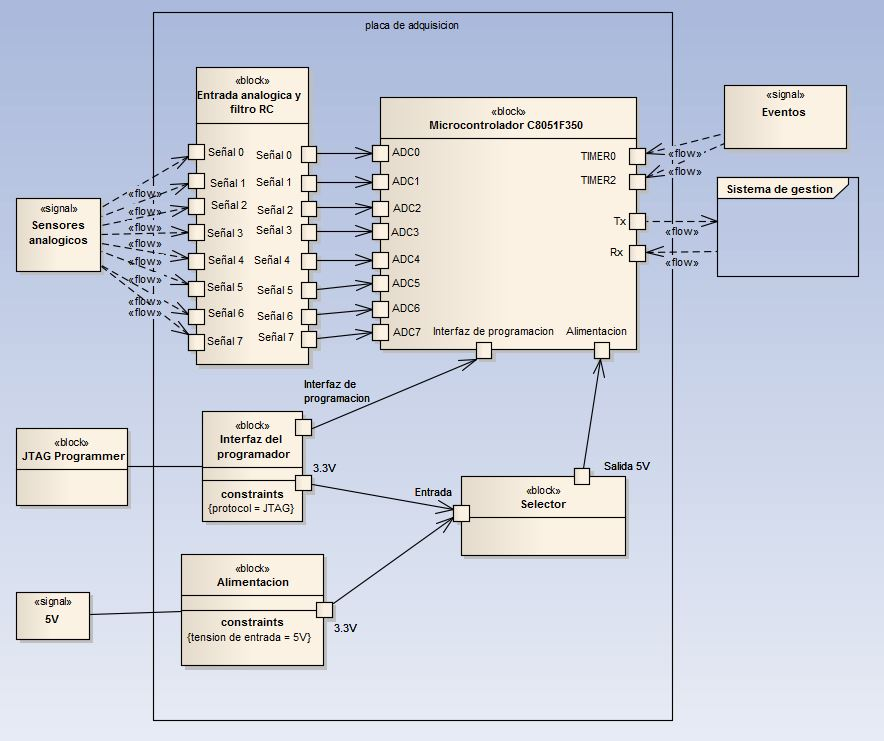
\includegraphics[width=0.80\textwidth, height = 11cm]{BloquesHardw1}
  \caption{Diagrama de Bloque de la Placa.}\label{fig:BloquesHardw1}
\end{figure}

Los bloques en la figura 5 representan de forma general los distintos módulos a implementar. Las entradas analógicas se introducen al sistema (microcontrolador) a través de filtros reductores del ruido (filtros RC). Luego, las señales, son procesadas por el microcontrolador (C8051f352). El bloque de GPIO y contadores de eventos es simplemente un grupo de pines direccionados a distintas entradas del microcontrolador, GPIO significa "General Purpose Input Output"(en español, "entrada y salida de propósito general" ). Son 4 pines que se separaron para uso general, por necesidad eventual de necesitarlos. Parte de estos GPIO son los pines contadores de eventos, por lo cual se incluyeron dentro del mismo bloque.

Es posible alimentar el sistema por medio del programador o debugger (propietario de Silicon Labs), o mediante una fuente de tensión externa de 5V, que al pasar por un regulador de tensión disminuye su voltaje a 3.3V para llegar al nivel de tensión del C8051f352. Ademas tendrá una llave selectora donde decidimos si se alimenta el sistema usando la fuente continua de 5V, o utilizando el programador.

%subsection diagra_bloques_hardware (end)

\subsection{Diseño Esquemático}
\label{diseno_esquematico}

Para poder realizar el diseño esquemático del circuito utilizamos el software KiCad. Para simplificar la explicación del diagrama, lo que haremos en esta sección es dividir el circuito entero en subcircuitos mas simples. Al final mostraremos el sistema final.

\subsubsection{Entradas Analógicas}
\label{entradas_analogicas}

El circuito contiene 8 entradas analógicas iguales cada una, por lo que mostraremos el ejemplo de una sola entrada. Podemos ver en la figura  el circuito para la entrada de la señal. 

Sabemos que la señal entra al sistema con ruido (ya sea como interferencia de señales externas, o ruido provocado por los mismos componentes del circuito). Por lo que como primera medida, se aplica a la señal de entrada un filtro RC pasivo, pasa bajo. Así introducimos muy poca atenuación a las frecuencias que son menores que la frecuencia de corte. Las frecuencias que son mayores que la de corte son atenuadas fuertemente. 
Como podemos ver en la figura \ref{fig:Entrada_y_filtro} tenemos un pin (AI0) de entrada para conectar la salida de un sensor analógico, seguido de un filtro RC, compuesto por una resistencia de 100 ohms, y un capacitor a tierra de 0,1 microFaradios. La salida de la resistencia esta conectada directamente a la entrada AIN0.0 del C8051f352.

\begin{figure}[h]
  \centering
  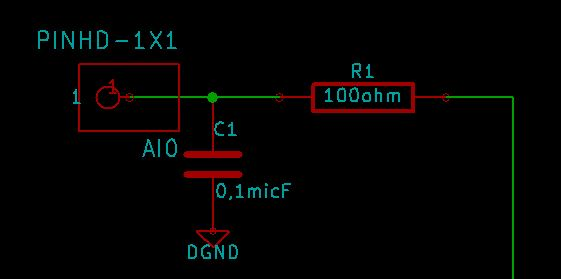
\includegraphics[width=0.80\textwidth, height = 11cm]{Entrada_y_filtro}
  \caption{Esquemático del circuito de entrada analógica, más filtro RC pasa-bajo.}\label{fig:Entrada_y_filtro}
\end{figure}

%subsubsection entradas_analogicas (end)

\subsubsection{Circuito Salida Serial}
\label{salida_serial}

Uno de los requerimientos de esta iteración es que la placa a desarrollar debe soportar comunicación serial, así que propusimos que dicha comunicación sea vía RS-232.

Como el nivel de tensión que entrega la salida serial TTL del microcontrolador C8051f352 es distinta a la necesaria para aplicar el protocolo RS-232. Nos vimos obligados a realizar un circuito para adaptarlo, y así asegurar el correcto envío de datos. Para realizar dicho circuito se utilizó el integrado MAX232 y se configuró como se muestra en la figura \ref{fig:MAX232}. Como podemos ver se utilizaron Capacitores de 0,1 microFaradios. Los pines "XRX1", "XCTS1", "XTX1" y "XRTS1" son los que tendrá el modulo de salida RS-232.
Ademas colocamos 4 jumpers (JP1, JP2, JP3, JP4) a la entrada del MAX232 por si se necesita la salida TTL del microcontrolador (por ejemplo si se quiere conectar la salida serial a un arduino o raspberry pi).

La tensión para alimentar el integrado es de 3.3V que se sacan del sub-circuito de potencia que se explicara en \ref{sub}.

\begin{figure}[h]
  \centering
  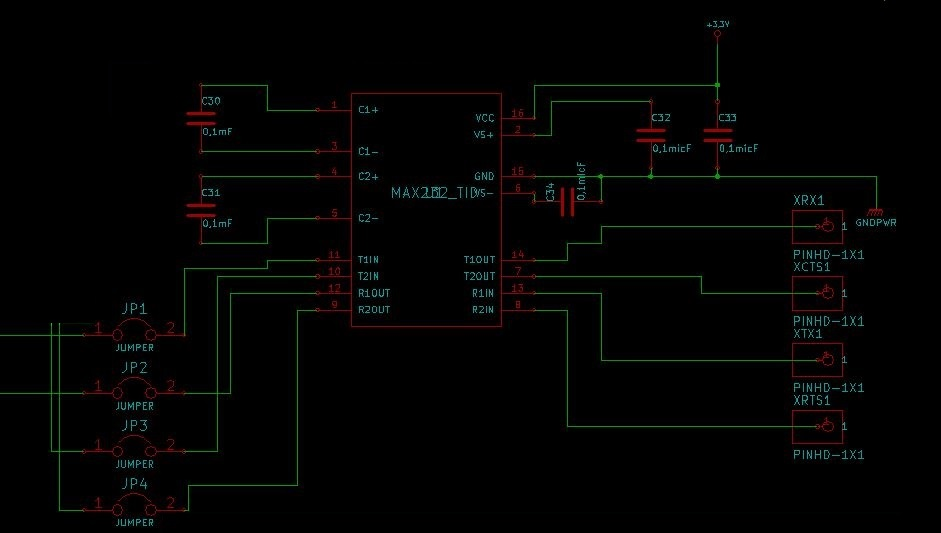
\includegraphics[width=0.80\textwidth, height = 11cm]{MAX232}
  \caption{Esquemático del Circuito MAX232 .}\label{fig:MAX232}
\end{figure}

%subsubsection salida_serial (end)

%subsection diseno_esquematico (end)

% section desarrollo (end)

\section{Pruebas} % (fold)
\label{sec:pruebas}

% section pruebas (end)

\section{Resultados} % (fold)
\label{sec:resultados}

% section resultados (end)

% chapter iteracion_3 (end)